
\documentclass[tikz,convert={convertexe={magick.exe}}]{standalone}
%\documentclass[tikz,convert]{standalone}
\usetikzlibrary{arrows}

\usepackage{ifthen}

\begin{document}
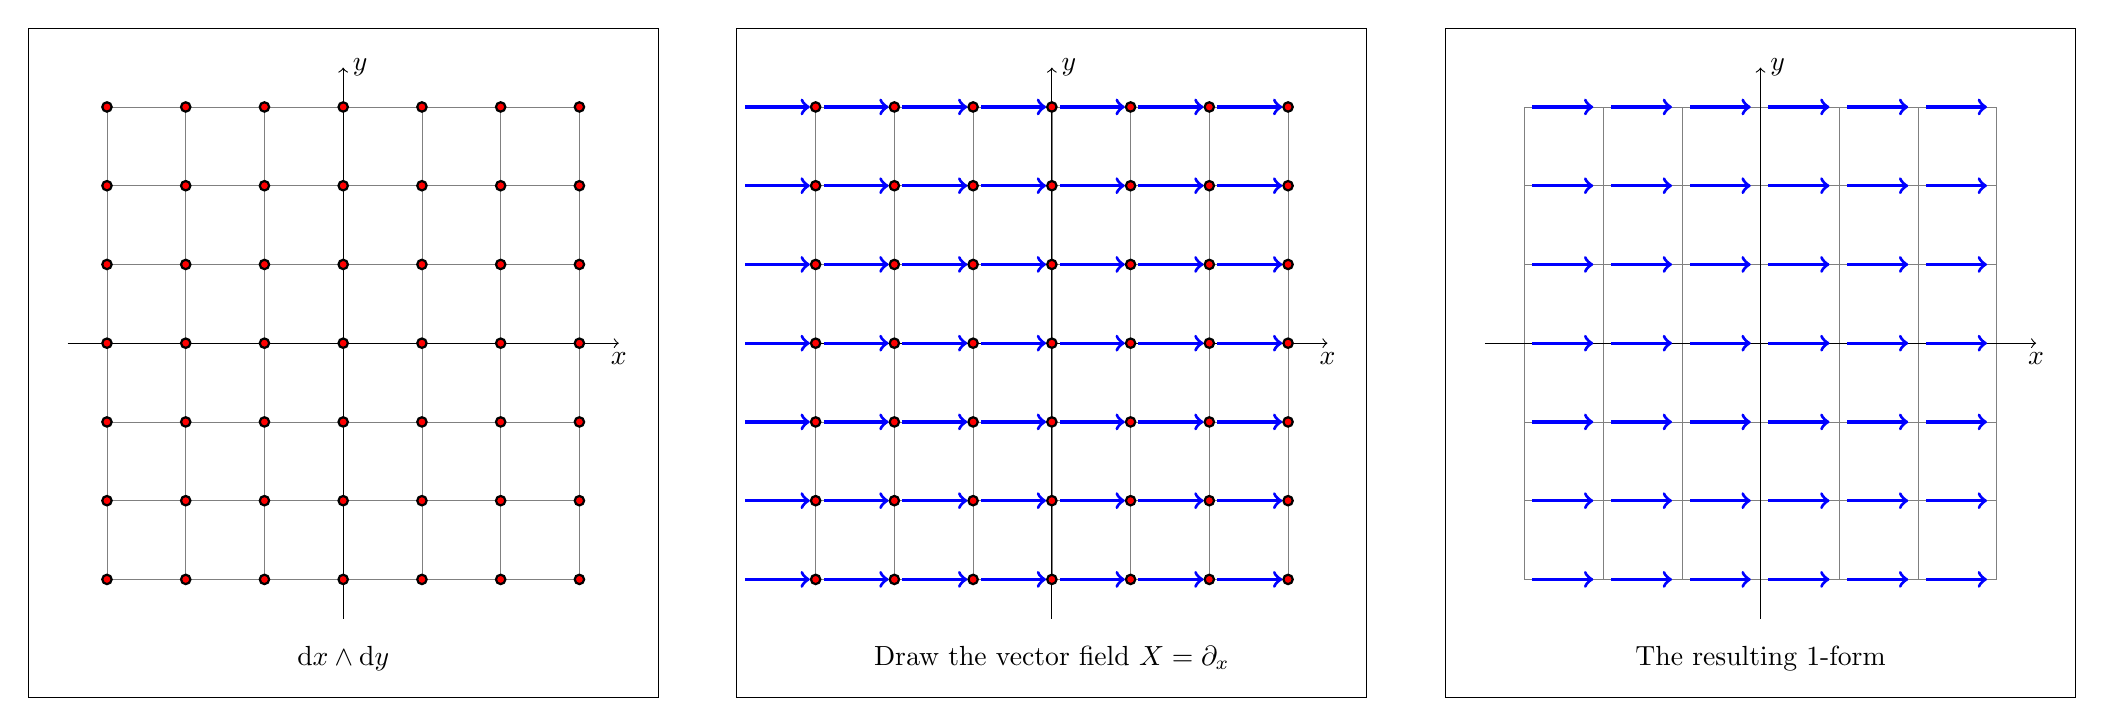
\begin{tikzpicture}

\tikzstyle atom=[circle, draw, inner sep=1.2pt, fill=red, thick]

\begin{scope}
\draw[style=help lines, very thin] (-3,-3) grid (3,3);

\draw[->] (-3.5,0)--(3.5,0) node[below] {$x$};
\draw[->] (0,-3.5)--(0,3.5) node[right] {$y$};

\draw (-4,-4.5) rectangle (4,4);
\node at (0,-4) {$\mathrm{d}x \wedge \mathrm{d}y$};

\foreach \x in {-3,...,3}
\foreach \y in {-3,...,3}
\node[atom] at (\x,\y) {};
\end{scope}

\begin{scope}[xshift=9cm]
\draw[style=help lines, very thin] (-3,-3) grid (3,3);

\draw[->] (-3.5,0)--(3.5,0) node[below] {$x$};
\draw[->] (0,-3.5)--(0,3.5) node[right] {$y$};

\draw (-4,-4.5) rectangle (4,4);
\node at (0,-4) {Draw the vector field $X = \partial_x$};

\foreach \x in {-3,...,3}
\foreach \y in {-3,...,3} {
\node[atom] (\x\y) at (\x,\y) {};
\draw[very thick,<-,blue] (\x\y) -- +(-.9,0);
}
\end{scope}

\begin{scope}[xshift=18cm]
\draw[style=help lines, very thin] (-3,-3) grid (3,3);

\draw[->] (-3.5,0)--(3.5,0) node[below] {$x$};
\draw[->] (0,-3.5)--(0,3.5) node[right] {$y$};

\draw (-4,-4.5) rectangle (4,4);
\node at (0,-4) {The resulting 1-form};

\foreach \x in {-2,...,3}
\foreach \y in {-3,...,3} {
\node[] (\x\y) at (\x,\y) {};
\draw[very thick,<-,blue] (\x\y) -- +(-.9,0);
}
\end{scope}

\end{tikzpicture}
\end{document}